\documentclass{standalone}
\usepackage{tikz}
\usepackage{verbatim}
\usetikzlibrary{positioning}
\begin{document}
\pagestyle{empty}
  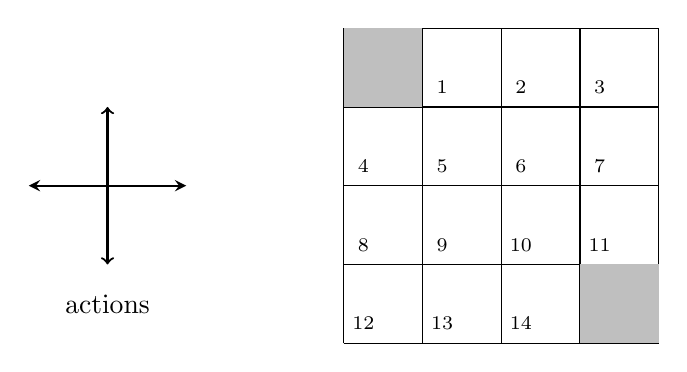
\begin{tikzpicture}
    \draw[stealth-stealth,thick] (-4, 2) -- (-2, 2);
    \draw[<->,thick] (-3, 1) -- (-3, 3);
    \node at (-3, 0.5) {actions};
    \draw[step=1.0,black,thin] (0,0) grid (4, 4);
    \fill[gray!50] (0, 3) rectangle (1,4);
    \fill[gray!50] (3, 0) rectangle (4,1);
    % Top row.
    \node at (1.25, 3.25) {\scriptsize 1};
    \node at (2.25, 3.25) {\scriptsize 2};
    \node at (3.25, 3.25) {\scriptsize 3};
    % Second frop top row.
    \node at (0.25, 2.25) {\scriptsize 4};
    \node at (1.25, 2.25) {\scriptsize 5};
    \node at (2.25, 2.25) {\scriptsize 6};
    \node at (3.25, 2.25) {\scriptsize 7};
    % Second from bottom row.
    \node at (0.25, 1.25) {\scriptsize 8};
    \node at (1.25, 1.25) {\scriptsize 9};
    \node at (2.25, 1.25) {\scriptsize 10};
    \node at (3.25, 1.25) {\scriptsize 11};
    % Bottom row.
    \node at (0.25, 0.25) {\scriptsize 12};
    \node at (1.25, 0.25) {\scriptsize 13};
    \node at (2.25, 0.25) {\scriptsize 14};
  \end{tikzpicture}
\end{document}